
\documentclass[a4paper, 14pt]{extarticle}
\usepackage[T2A]{fontenc}
\usepackage[utf8]{inputenc}
\usepackage[russian]{babel}
\usepackage{geometry}
\usepackage{amsmath, amssymb, mathtext, graphicx}
\usepackage{setspace}
\usepackage{titlesec}
\usepackage{caption}

\geometry{left=3cm, right=1.5cm, top=2cm, bottom=2cm}
\onehalfspacing
\setlength{\parindent}{1.25cm}

\titleformat{\section}{\newpage\centering\normalfont\large\bfseries}{\thesection}{1em}{}
\titleformat{\subsection}{\normalfont\normalsize\bfseries}{\thesubsection}{1em}{}

\captionsetup[figure]{labelsep=endash, justification=centering, name=Рисунок}

\begin{document}
	
	% --- ТИТУЛЬНЫЙ ЛИСТ ---
	\begin{titlepage}
		\centering
		\singlespacing % На титульном листе интервал обычно одинарный
		{\small МИНИСТЕРСТВО НАУКИ И ВЫСШЕГО ОБРАЗОВАНИЯ \\ РОССИЙСКОЙ ФЕДЕРАЦИИ\\
			МОСКОВСКИЙ ФИЗИКО-ТЕХНИЧЕСКИЙ ИНСТИТУТ\\
			(НАЦИОНАЛЬНЫЙ ИССЛЕДОВАТЕЛЬСКИЙ УНИВЕРСИТЕТ)\\
			\vspace {1cm}
			Кафедра вакуумной электроники\\}
		
		\vspace{4cm}
		
		Лабораторная работа \\
		по курсу Вакуумная электроника\\
		{\Large \textbf{Напыление тонких плёнок в вакууме}\\}
		
		\vspace{3cm}
		
		% Блок с исполнителем и преподавателем
		\begin{flushright}
			\begin{minipage}{0.45\textwidth}
				\raggedright
				Выполнил: \\
				студент группы Б04-507 \\
				Рудачихин П.А. \\
				\vspace{0.5cm}
				Преподаватель: \\
				... \\
				\vspace{0.5cm}
				Дата выполнения: 16.09.2026
			\end{minipage}
		\end{flushright}
		
		\vfill
		
		Долгопрудный \\
		2026
	\end{titlepage}
	
	% --- ОСНОВНАЯ ЧАСТЬ ---
	% Согласно ГОСТ, структурные элементы (ВВЕДЕНИЕ, ЗАКЛЮЧЕНИЕ и т.д.) пишутся прописными буквами
	\section*{АННОТАЦИЯ} % Если нужно, можно добавить в содержание
	\addcontentsline{toc}{section}{АННОТАЦИЯ}
	
	Цель настоящей работы -- ознакомление с методами термовакуумного напыления тонких плёнок. Производится термовакуумное напыление алюминиевой плёнки на стеклянную пластинку, измеряется толщина плёнки оптическим методом.
	
	\section*{ВВЕДЕНИЕ}
	\stepcounter{section}
	\addcontentsline{toc}{section}{ВВЕДЕНИЕ}
	
	Рассмотрим простейшую модель термовакуумного напыления с резистивным испарителем. Испаряемое вещество находится в виде маленькой капли (точечный источник) непосредственно на испарителе, который нагревается пропускаемым через него током. Над испарителем на расстоянии $R$ горизонтально расположена плоскость подложки.
	
	\subsection{Требования к вакууму}
	
	Для качественного формирования плёнки важно минимизировать появление частиц остаточных газов в пространстве между испарителем и подложкой, т.е. длина свободного пробега остаточных газов $\lambda$ должна быть много больше $R$. Предположим, что частицы остаточных газов с концентрацией $n$ и давлением $P$ имеют одинаковые радиус $r$ и температуру $T_0$, тогда
	
	\begin{equation}
		\lambda = \frac{1}{\sqrt{2}\cdot n\cdot 4\pi r^2} = \frac{kT_0}{4\sqrt{2}\pi P r^2}
	\end{equation}	
	
	Подставив средний радиус частиц воздуха $r = 0,187$ нм и комнатную температуру $T= 298$ К, получаем
	
	\begin{equation}
		\lambda \approx \frac{6,62\cdot 10^{-3}}{P}, \ \ \ \lambda(\text{см}) \approx \frac{8,71\cdot 10^{-3}}{P(\text{Торр})}
	\end{equation}	
	
	\subsection{Толщина плёнки}
	
	Считая испарение изотропным, можно ввести массовый поток 
	
	\begin{equation}
		\mu := \frac{dm}{Sdt} = \frac{\dot{m}}{4\pi r^2}
	\end{equation} 
	
	где $r$ -- расстояние до источника.
	
	\begin{figure}[h!]
		\centering
		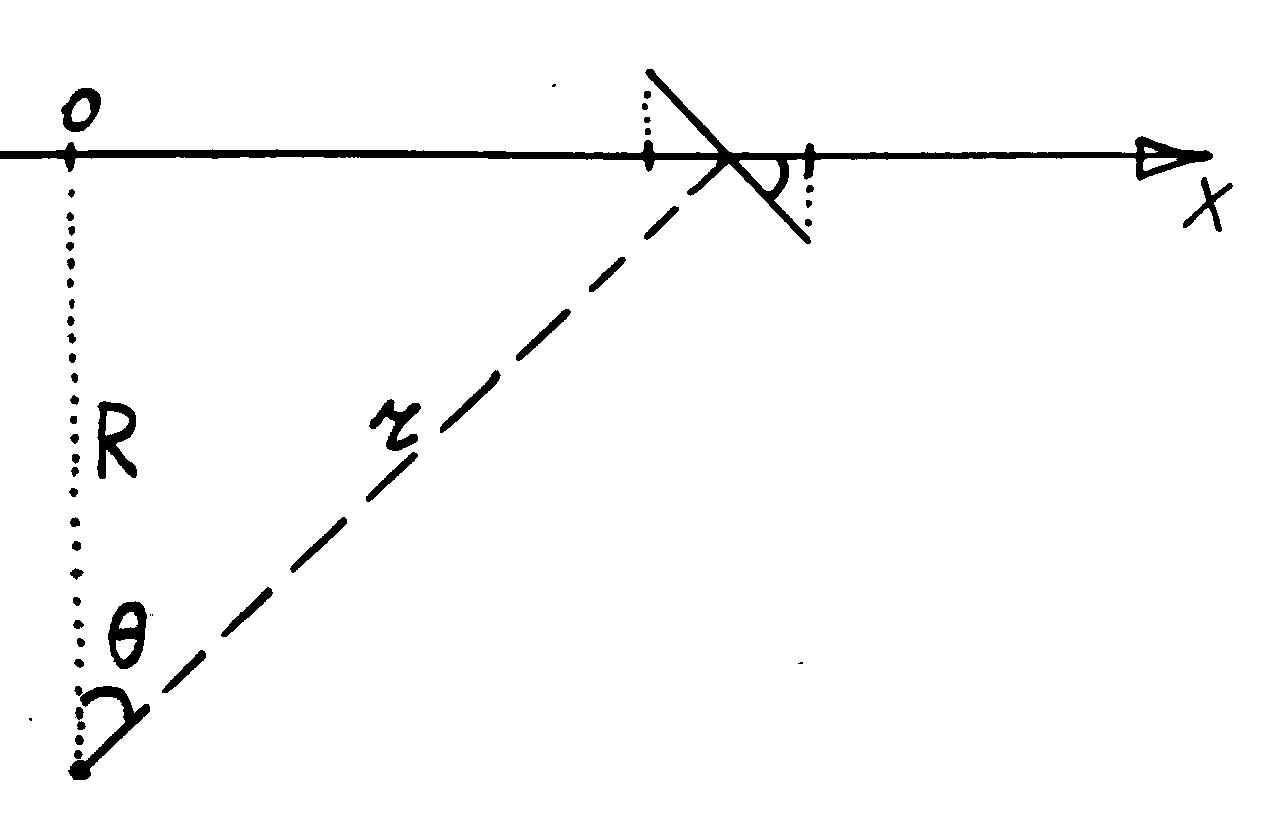
\includegraphics[width=0.4\linewidth]{scheme1}
		\caption{Геометрия напыления}
		\label{fig:scheme1}
	\end{figure}
	
	Из геометрических соображений (см. рис. \ref{fig:scheme1}) $r^2 = R^2 + x^2$, $dS_x = dS/\cos\theta$. Поток массы на плоскости
	
	\begin{equation}
		\mu_x := \frac{dm}{dS_x dt} = \mu \cos\theta = \frac{\dot{m}}{4\pi}\frac{R}{(R^2 + x^2)^{3/2}}
	\end{equation} 
	
	С другой стороны, приняв во внимание $dV = dh \cdot dS_x$, имеем
	
	\begin{equation}
		\mu_x := \frac{dm}{dS_x dt} = \frac{\rho dV}{dS_x dt} = \rho \dot{h}
	\end{equation} 
	
	Получаем уравнение
	
	\begin{equation}
		\dot{h} = \frac{\dot{m}}{4\pi\rho}\frac{R}{(R^2 + x^2)^{3/2}}
	\end{equation}
	
	Его решение:
	
	\begin{equation}
		h = \frac{m}{4\pi\rho}\frac{R}{(R^2 + x^2)^{3/2}}
	\end{equation}
	
	Аддитивной константы нет, так как на бесконечности $h=0$. В частности, в ближайшей к источнику точке плоскости
	
	\begin{equation}
		h_0 = \frac{m}{4\pi\rho R^2}
	\end{equation}
	
	\begin{figure}[h!]
		\centering
		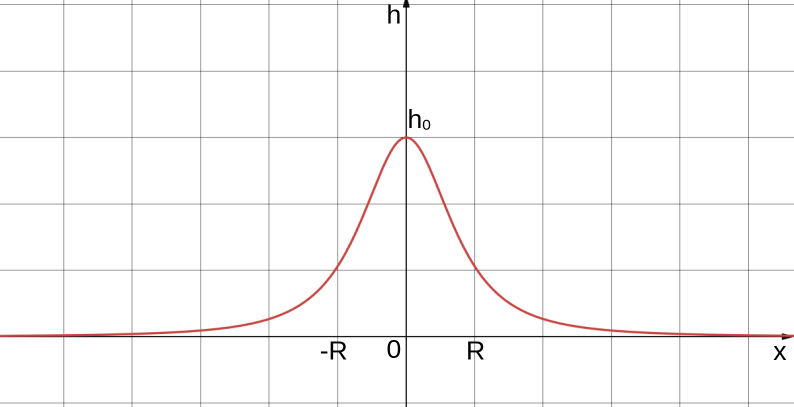
\includegraphics[width=0.8\linewidth]{graph1}
		\caption{График $h(x)$}
		\label{fig:graph1}
	\end{figure}
	
	Построим график, отражающий распределение толщины по плоскости на расстоянии $x$ от ближайшей к испарителю точки $x=0$ (см. рис. \ref{fig:graph1})
	
	\begin{equation}
		h(x) = h_0(1 + (x/R)^2)^{-3/2}
	\end{equation}
	
	\subsection{Особенности резистивного испарителя}
	
	В данной работе используется резистивный тип испарителя, поэтому необходимо, чтобы температура плавления испарителя была выше температуры испаряемого вещества, давление паров материала испарителя было много меньше давления паров испаряемого вещества, материалы испарителя и испаряемого вещества не вступали в химическую реакцию. Испаряемое вещество должно смачивать испаритель, чтобы обеспечить хороший тепловой контакт и механическую стабильность.
	
	\subsection{Оптический контроль толщины}
	
	Плёнка алюминия полупрозрачна при толщине 5 -- 30 нм, и в этом диапазоне для определения её толщины можно использовать закон Бугера-Ламберта-Бера:
	
	\begin{equation}
		I_{out} = I_{in} \cdot \exp(-\frac{4\pi k}{\lambda} h)
	\end{equation}
	
	где $I_{out}$ -- интенсивность света через стекло с напылением, $I_{in}$ -- интенсивность света через непокрытое стекло, $k = 5,2762$ -- показатель поглощения алюминия. Получаем формулу контроля толщины плёнки:
	
	\begin{equation}
		h = -\frac{\lambda}{4\pi k} \ln{\frac{I_{out}}{I_{in}}} 
	\end{equation}
	
	Однако показатель поглощения алюминия зависит от длины волны света, поэтому в работе толщина плёнки оценивается по эмпирическим данным с сайта RefractiveIndex.INFO: Cheng et al, где для разных толщин $h$ получена зависимость пропускания от длины волны $T(\lambda)$. 
	
	\section{ОПИСАНИЕ УСТАНОВКИ}
	
	\begin{figure} [h!]
		\centering
		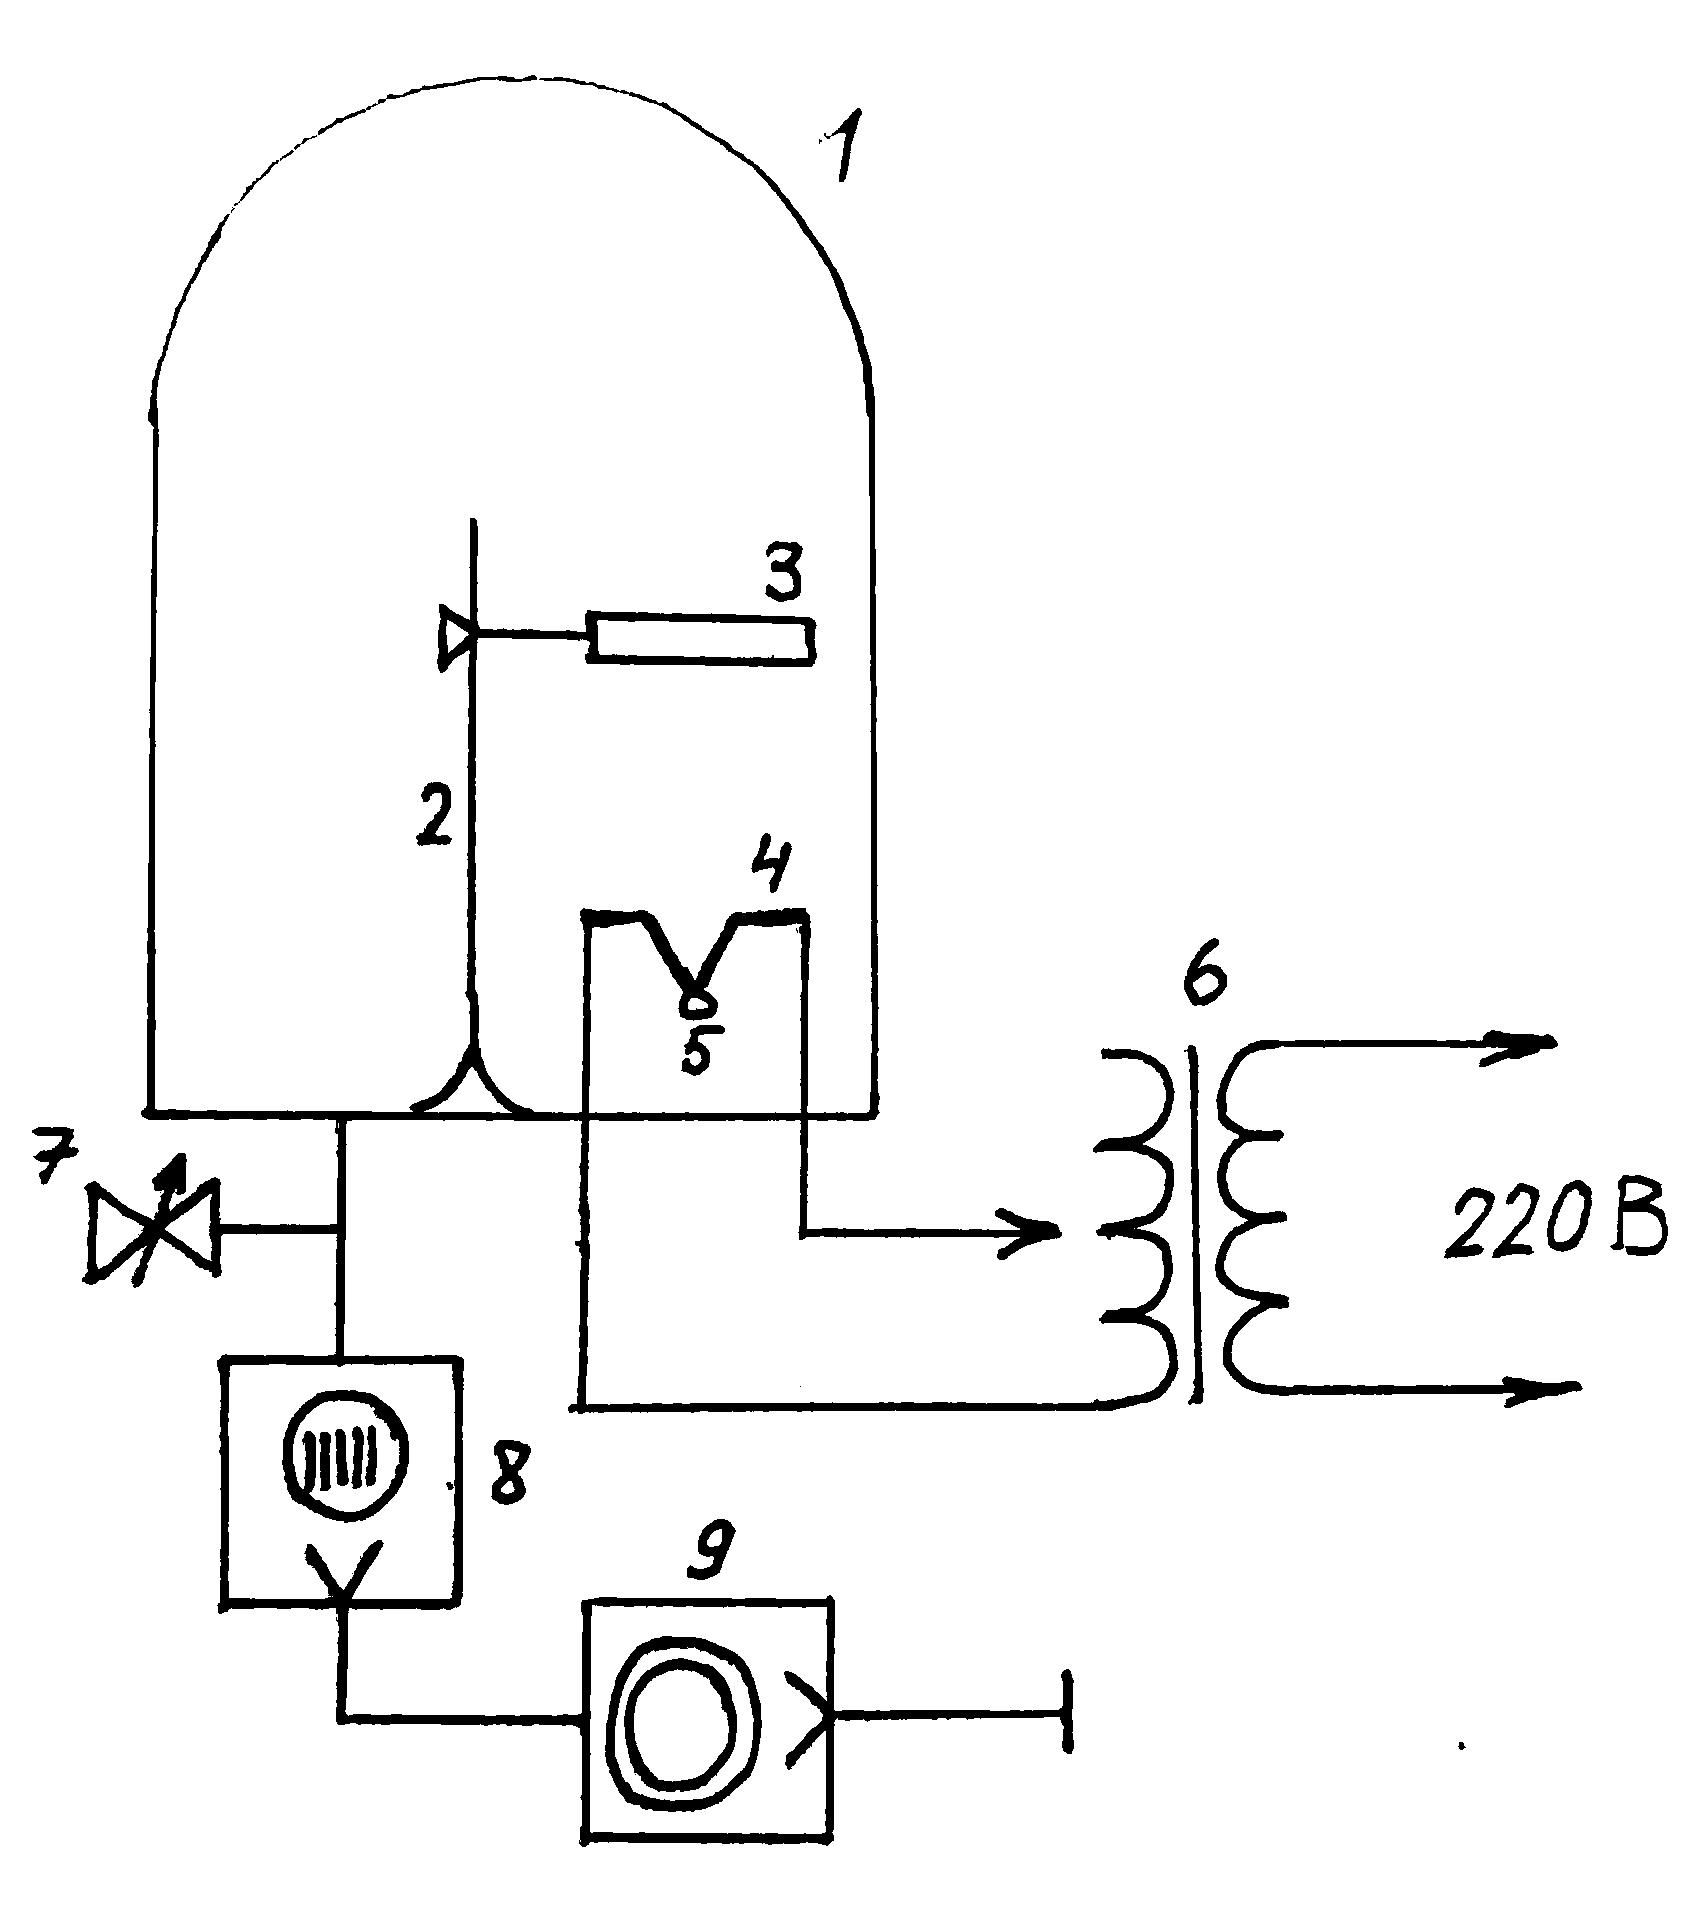
\includegraphics[width=0.7\linewidth]{setup}
		\caption{Упрощённая схема установки: 1 -- вакуумный колпак, 2 -- штатив, 3 -- стеклянная пластинка, 4 -- вольфрамовый испаритель, 5 -- образец алюминия, 6 -- трансформатор, 7 -- натекатель, 8 -- турбомолекулярный насос, 9 -- форвакуумный насос}
		\label{fig:setup}
	\end{figure}
	
	Упрощённая схема установки представлена на рисунке \ref{fig:setup}. Вакуумная система состоит из колпака 1, натекателя 7, турбомолекулярного 8 и форвакуумного 9 насосов. Напыление происходит на стеклянную пластинку 3. Она зафиксирована штативом 2 на расстоянии $R$ от образца алюминия 5, находящегося на вольфрамовом испарителе 4. Испаритель подключён к трансформатору 6, с помощью которого регулируется ток через испаритель.
	
	Для измерения пропускания стеклянной пластинки используется специальное устройство, состоящее из источника света, фотоприёмника и электронного блока с многоразрядным семисегментным светодиодным индикатором. Погрешность принята равной 3 единицам последнего разряда.
	
	Для измерения расстояния $R$ от испарителя до стекла и длины $l$ алюминиевой проволоки использована линейка с погрешностью 0,5 мм. 
	
	Диаметр $d$ алюминиевой проволоки измерен штангенциркулем с погрешностью 0,05 мм.
	
	\section{ПРЕДВАРИТЕЛЬНЫЕ ИЗМЕРЕНИЯ И РАСЧЁТЫ} 
	
	Расстояние $R$ порядка 10 см. Длина свободного пробега остаточных газов такого порядка соответствует давлению $P \sim 10^{-3}$ Торр.
	
	Образец алюминия нарезается из алюминиевой проволоки диаметром \[ d = (0,30 \pm 0,05) \ \text{мм} \] и размещается на расстоянии \[ R = (130 \pm 1) \ \text{мм} \] от подложки. Рассчитаем длину проволоки, необходимую для напыления $h_0 = 25$ нм:
	
	\begin{equation}
		l = \frac{V}{S} = \dfrac{4m}{\rho\pi d^2} = \frac{4 \cdot 4\pi\rho h_0 R^2}{\rho \pi d^2} = 16 h_0 \frac{R^2}{d^2} \approx 8 \text{ см}
	\end{equation}
	
	Проволока отрезана по этим размерам: \[ l = (80 \pm 1) \ \text{мм} \] 
	
	Ожидаемая толщина плёнки
	
	\begin{equation}
		h =  \frac{l d^2}{16 R^2} = (27 \pm 4)  \text{ нм} 
	\end{equation}
	
	\section{ХОД РАБОТЫ}
	
	Откачка происходит при одновременной работе турбомолекулярного и форвакуумного насосов. Возвращение к атмосферному давлению происходит после выключения форвакуумного и полной остановки турбомолекулярного насоса открыванием натекателя. Оценка температуры испарителя производится по цвету каления: 660 $^o$С -- тёмно-красное, 1150 $^o$С -- жёлтое, 1500 $^o$С -- светло-жёлтое.
	
	Первая попытка напылить алюминиевую плёнку толщиной 5 мм обернулась неудачей -- не было зафиксировано изменение интенсивности света через пластинку. Приведём ход работы при второй попытке. 
	
	\begin{enumerate}
		\item Вольфрамовая проволока первично очищена от графитовой смазки с помощью бумажной салфетки, смоченной в деионизированной воде.
		\item Аналогично очищены контактные площадки, уплотнители, колпак и штатив.
		\item Вольфрамовой проволоке придают форму литеры <<V>> и подключают к контактам. 
		\item В вакууме порядка $10^{-2}$ Торр вольфрамовая проволока раскаляется до светло-жёлтого цвета, чтобы очистить и обезгазить её.
		\item На испаритель размещается образец алюминия.
		\item По достижении вакуума $1,3 \cdot 10^{-3}$ Торр начато напыление.
		\item Установлена температура испарителя около 660 $^o$С: образец алюминия постепенно плавится, смачивает испаритель и образует каплю.
		\item На 10 -- 20 с температура испарителя поднимается до 1150 $^o$С -- происходит испарение алюминия.
		\item После приведения установки к атмосферному давлению имеем стеклянную пластинку с напылённой плёнкой алюминия.
		\item Измеряем толщину плёнки оптическим методом.
	\end{enumerate} 
	
	\section{РЕЗУЛЬТАТЫ И ОБСУЖДЕНИЯ}
	
	Причиной неудачи в первой попытке могло стать недостаточное количество алюминия: уже при его предварительном плавлении и смачивании часть вещества испарилась, не достигнув пластинки. Во второй попытке напыления количество алюминия и ожидаемая толщина плёнки были увеличены. 
	
	Интенсивности света через стеклянную пластинку без напыления и с напылением составили соответственно
	
	\[ I_{in} = (1293 \pm 3) \text{ усл.ед.} \ \ \ I_{out} = (59 \pm 3) \text{ усл.ед.} \]
	
	Коэффициент пропускания составил
	
	\[ T = \frac{I_{out}}{I_{in}} = 0,046 \pm 0,002 \]
	
	\begin{figure}[h!]
		\centering
		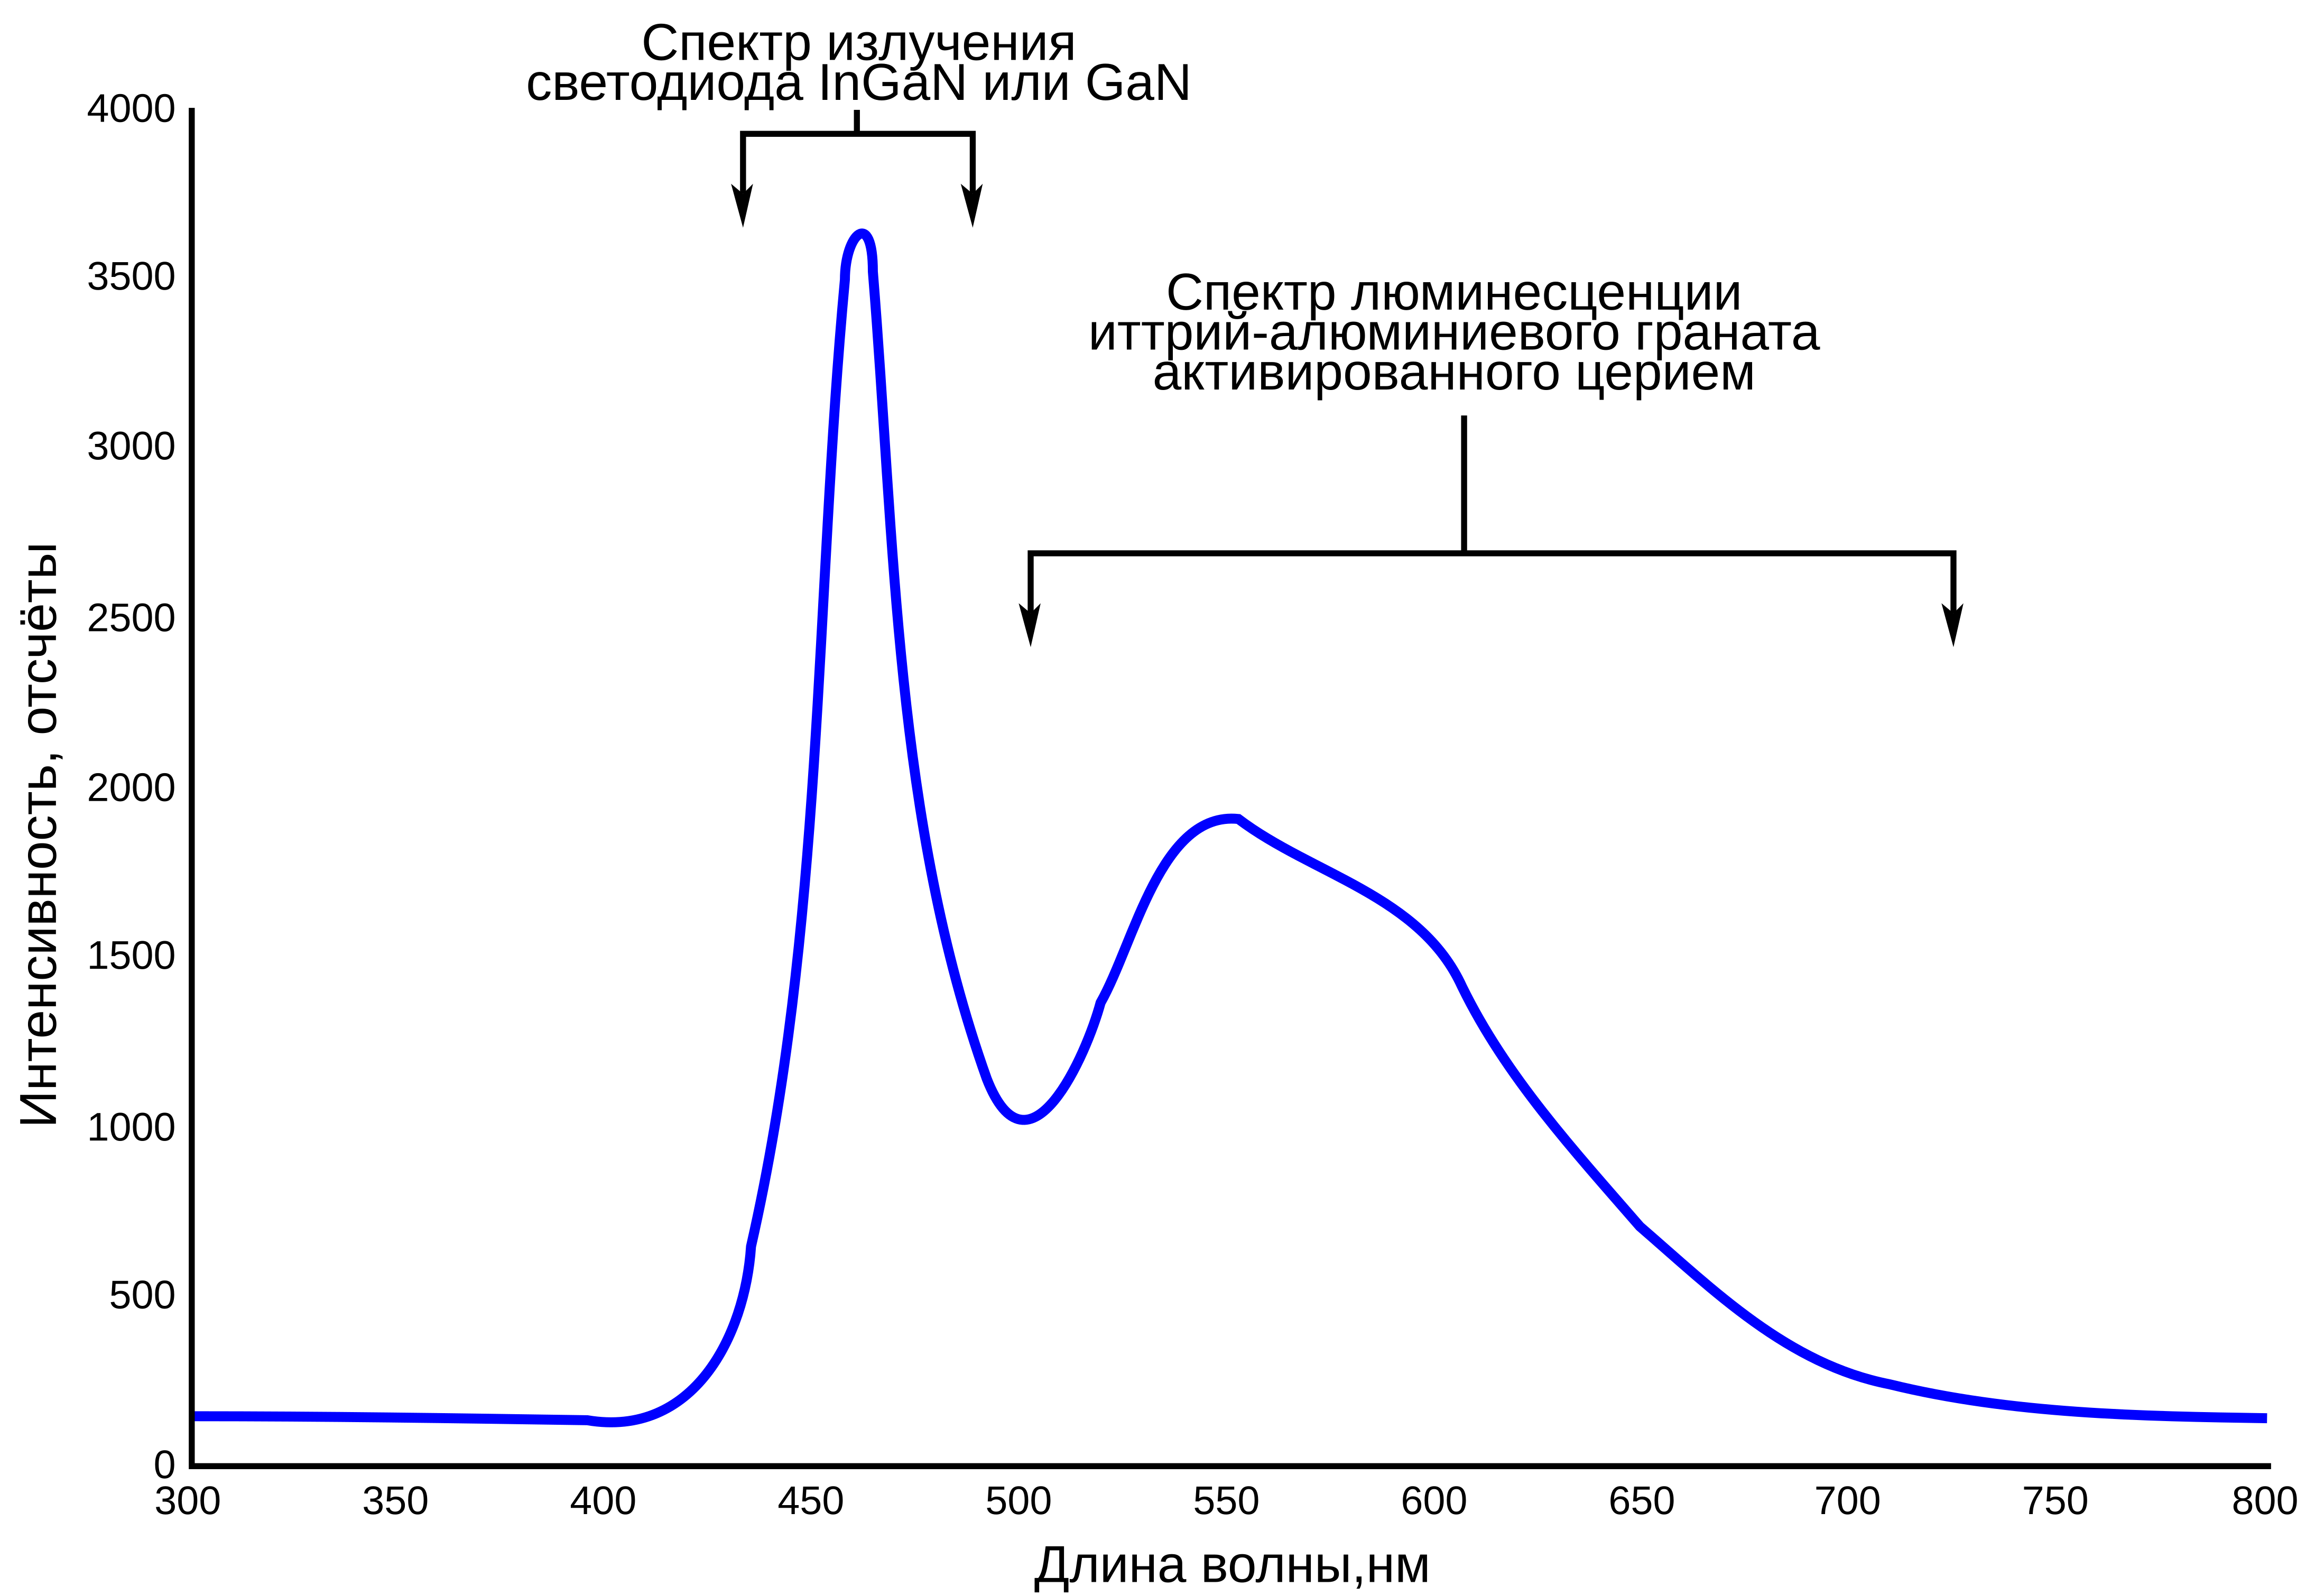
\includegraphics[width=0.7\linewidth]{led}
		\caption{Спектр белого светодиода}
		\label{fig:led}
	\end{figure}
	
	В приборе для измерения интенсивности в качестве источника света выступает белый светодиод. Его спектр (см. рис. \ref{fig:led}) имеет максимум на длине волны 460 нм. Для неё с помощью данных сайта RefractiveIndex.INFO перебором найден диапазон значений $h$, соответствующий измеренному $T$:
	
	\[ h = (25,7 \pm 0,4) \text{ нм} \]
	
	Этот диапазон полностью входит в доверительный интервал ожидаемого значения $h$, но его среднее 25,7 нм меньше расчётных 27 нм. Занижение контрольного значения обусловлено его усреднением  по области прохождения светового луча. Между тем, расчётная толщина достигается только в точке, ближайшей к источнику. Кроме того, на результат может влиять анизотропия испарения и остаточные газы, которые сокращают число молекул алюминия достигающих пластинки.
	
	\section*{ЗАКЛЮЧЕНИЕ}
	\addcontentsline{toc}{section}{ЗАКЛЮЧЕНИЕ}
	
	Первая попытка напыления алюминия оказалась неудачной. Анализ этой ситуации позволил после некоторых изменений хода работы  и условий эксперимента (прежде всего, увеличения количества алюминия) получить напылённую на стекло алюминиевую плёнку. Её толщина, определённая оптическим методом, составила 25,7 нм. 
	
\end{document}